\section{Método dos Elementos Finitos}

Para \citep[p. 19]{jin}, o método dos elementos finitos é uma técnica numérica para se obter soluções aproximadas de problemas de valor de contorno.

Para \citep[p. 13]{reddy}, o MEF trata-se de um método no qual o domínio do problema é visto como uma coleção de subdomínios, sobre os quais, a equação que modela o problema é aproximada por um método variacional.

Segundo \citep[p. 19]{jin},  o método foi desenvolvido inicialmente para a aplicação em análise estrutural, mas em seguida foi estendido para solucionar problemas de outros campos.

Como foi dito anteriormente, problemas contínuos se tornam intratáveis à medida em que a complexidade aumenta. 
A fim de atacar este problema, foram desenvolvidas por matemáticos, engenheiros e cientistas, estratégias de discretização do domínio e aproximação dos valores da solução. 
\citep[p. 1]{zien}

Enquanto matemáticos desenvolveram técnicas aplicáveis diretamente sobre as equações diferenciais que governam o problema, tais como o método dos resíduos ponderados e a minimização de funcionais, os engenheiros adotaram abordagens mais intuitivas, por meio da analogia entre elementos discretos e porções finitas de um domínio contínuo.
\citep[p. 1]{zien}

Uma vez que se têm métodos para a discretização e para a aproximação da solução, é possível definir o método dos elementos finitos como sendo uma sequência de passos para a resolução de problema físico ou matemático a partir de um modelo discreto mais simples (ou relaxado) do problema original. O novo modelo é chamado de formulação fraca, e é geralmente dado na forma integral. O modelo original descrito por equação diferencial é denominado formulação forte. \textbf{***REF}

\subsection{Visão geral}
A aplicação do MEF compreende basicamente três etapas: pré-processamento, análise e pós-processamento. Cada etapa apresenta uma contribuição para que se obtenha um resultado satisfatório. O pré-processamento é responsável pela discretização e por estabelecar as restrições físicas do domínio. A etapa de análise obtém a aproximação do modelo (forma fraca), e aplica esta aproximação em cada sub-domínio. O resultado preliminar da análise é um sistema de equações lineares que quando resolvido, fornece a solução do problema.  O pós-processamento consiste na exibição adequada dos resultados.A seguir cada etapa é vista em detalhes.



\subsubsection{Pré-Processamento}

A etapa de pré-processamento compreende a maior parte do tempo de modelagem do método. É neste ponto do processo que se são definidos os apectos geométricos do modelo, as propriedades dos materiais do objeto de estudo e a aplicação das condições de contorno ou condições iniciais.

\paragraph{Aspectos geométricos \\} 
A definição dos aspectos geométricos consiste na tranformação do domínio contínuo $\Omega$ em uma malha de elementos finitos. Cada elemento $\Omega_e$ dessa malha é um subdomínio de $\Omega,$. A figura \ref{fig:malhas} contém a representação de diferentes malhas propostas para o mesmo dominio $\omega$. A primeira e a segunda malha são uniformes, pois contém elementos de um único tipo, triângulos ou quadradados. Já a terceira malha é mista, pois apresenta elementos de ambos os tipos. 

\begin{figure}[!htb]
\centering
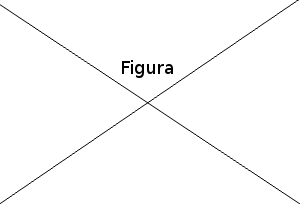
\includegraphics[scale=0.5]{figuras/temp.png}
\caption{Diferentes malhas para o domínio $\Omega$}
\label{fig:malhas}
\end{figure}

Cada elemento pode ser identificado na malha a partir de um número que lhe é atribuído. Na figura \ref{fig:numeracao}, os números entre parêntesis identificam os elementos.

Os vértices de uma elemento são chamados de nós. cada nó possui dois números vinculados a ele. Os índices na cor azul representam a numeração do nó dentro de um dado elemento (Identificação local). Os índices em vermelho por sua vez são os identificadores globais dos nós ao longo de toda a malha. Cada nó apresenta um determinado grau de liberdade dado pelo número máximo de componentes de um deslocamento. No exemplo de duas dimensões, cada nó tem no máximo 2 graus de liberdade, pois podem se deslocar nas direções de x e de y. O nó 1, no entanto, não apresenta graus de liberdade, pois está fixo. 

Os graus de liberdade de um elemento é a soma dos graus de liberdade de seus nós, dessa forma, um elemento triangular, por exemplo, no espaço bidimensional, possui no máximo 6 graus de liberdade.

\begin{figure}[!htb]
\centering
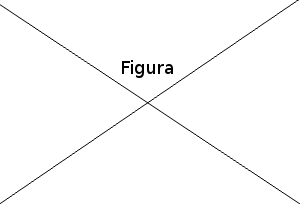
\includegraphics[scale=0.5]{figuras/temp.png}
\caption{Identificadores de Elementos e nós}
\label{fig:numeracao}
\end{figure}

\paragraph{Propriedades do material \\}
Para que o MEF seja capaz de aproximar adequadamente a solução de um problema, é necessário, além da geometria, se especificar as propriedades dos materiais em cada elemento da malha. Na análise estrutural, por exemplo, diferentes materiais reagem diferentemente à uma dada deformação ou  deslocamento, devido à sua rigidez e aos diferentes fenômenos que podem ocorrer, como por exemplo, fenômenos plásticos ou elásticos. Na análise eletromagnética, as propriedades dos materiais podem ser dadas em termos por exemplo, de condutividade, resistividade ou permissividade. Na análise térmica, algumas propriedades relevantes são o calor específico, a condutividade térmica e a expansão térmica.
Desta forma, de acordo com a área de análise, os materiais apresentam características determinantes para a obtenção de resultados adequados.

As propriedades dos materiais podem ainda estar condicionadas à uma determinada direção. Desta forma, os materiais podem ainda ser classificados como isotrópicos, anisotrópicos ou ortotrópicos. Materiais isotrópicos apresentam as mesmas propriedades físicas em todas as direções. Nos materiais anisotrópicos, as propriedades variam conforme a direção considerada. Nos materiais ortotrópicos, as propriedades são diferentes em direções perpendiculares entre si, formando eixos de ortotropia.

A título de exemplo, a tabela \ref{tab:permissividade} contém a comparação entre a permissividade relativa de diferentes materiais.

\begin{table}	
	\centering
	\begin{tabular}{|c|c|}	

	\end{tabular}
	\caption{A permissividade elétrica dos materiais}
	\label{tab:permissividade}
\end{table}


\paragraph{Valores de Contorno \\}
A atribuição dos valores de contorno é o último passo da etapa de pré- processamento. Estes valores são atribuídos a pontos específicos da malha e são importantes para caracterizar a unicidade de solução.

Considere um capacitor de placas paralelas, no qual uma das armaduras é submetida à uma tensão de 10V e outra à 0V. A ditribuição de potencial e o valor do campo elétrico entre as placas e no ambiente em volta do capacitor, podem ser definidos unicamente a partir das condições de contorno (10V e 10V) impostas em pontos (ou nós) específicos do domínio, como mostra a figura \ref{fig:capacitor}.

\begin{figure}[!htb]
\centering
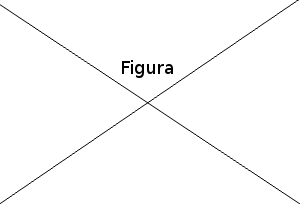
\includegraphics[scale=0.5]{figuras/temp.png}
\caption{Distribuição do potencial e o campo elétrico no capacitor de placas paralelas}
\label{fig:capacitor}
\end{figure}

\subsubsection{Processamento ou Análise de Elementos Finitos}
A etapa de processamento de elementos finitos consiste na elaboração de funções aproximadas para o modelo em questão. Essas aproximações devem ser feitas dentro de cada sub-domínio do sistema. A forma forte do problema é geralmente fornecida como uma equação ou sistemas de equações diferenciais e deve ser transformada no processamento em um conjunto de equações algébricas contínuas por partes.

\paragraph{Funcionamento do método \\}
Existem diferentes técnicas para a obtenção da forma fraca de uma equação diferencial. Os métodos tradicionalmente utilizados no MEF são os métodos de Ritz (Variacional) e de Galerkin (Resíduos ponderados). Mesmo com estes diferentes caminhos, os quais serão vistos mais à frente, FEM possui uma interpretação única, independente da  técnica de aproximação utilizada. 

Considere a malha bidimensional  apresentada na figura \ref{fig:malhaGenerica}. Esta malha pode representar por exemplo, a abstração de uma ponte metálica, de dutos de um fluido ou até mesmo um circuito elétrico, como apresentado na figura \ref{fig:repMalhaGenerica}.
\begin{figure}[!htb]
\centering
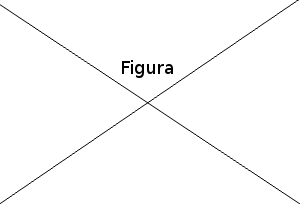
\includegraphics[scale=0.5]{figuras/temp.png}
\caption{Malha Genérica}
\label{fig:malhaGenerica}
\end{figure}

\begin{figure}[!htb]
\centering
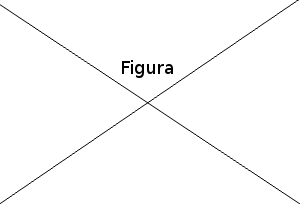
\includegraphics[scale=0.5]{figuras/temp.png}
\caption{Possíveis objetos de representação da malha \ref{fig:malhaGenerica}}
\label{fig:repMalhaGenerica}
\end{figure}


 Fazendo uma analogia com uma estrutura metálica, conforme apresentado na figura \ref{fig:repMalhaGenerica}-a, as forças que atuam nos nós, podem ser definidas  a a partir dos deslocamento destes nós, da distribuição da carga sobre um dado elemento e da tensão inicial, caso haja.
 
 Supondo que um carregamtno $p$ atue sobre o elemento $1$, as forças que atuam sobre os nós deste elemento podem ser dadas por:
 
 
 \begin{equation}
 	\label{eq:forca}
 	\begin{tabular}{c c}
 	$q_1 = 
		\left \{
 		\begin{tabular}{c}
	 		$q_1^1$ \\
	 		$q_2^1$ \\
	 		$q_3^1$
  		\end{tabular} 		
		\right \}$
		\
 	$q_1^1 = 
		\left \{
 		\begin{tabular}{c}
	 		$U_1$ \\
	 		$V_1$
  		\end{tabular} 		
		\right \}	$
		\end{tabular} 	
 \end{equation}


Similarmente, os deslocamentos podem ser dados para cada nó do elemento. Se as componentes da força na direção de x e y são dadas como U e V, as componentes da força podem ser dadas em função dessas componentes de deslocamento.

 \begin{equation}
 	\label{eq:desloc}
 	\begin{tabular}{c c}
 	$u_1 = 
		\left \{
 		\begin{tabular}{c}
	 		$u_1^1$ \\
	 		$u_2^1$ \\
	 		$u_3^1$
  		\end{tabular} 		
		\right \}$
		\
 	$u_1^1 = 
		\left \{
 		\begin{tabular}{c}
	 		$u_1(U_1)$ \\
	 		$v_1(V_1)$
  		\end{tabular} 		
		\right \}	$
		\end{tabular} 	
 \end{equation}


Assumindo um material isotrópico, cujo comportamento é linear elástico, a lei de Hooke fornece a equação \ref{eq:hooke}

 \begin{equation}
 	\label{eq:hooke}
	\textbf{$q^1 = K^1 u^1 + f^1$}
 \end{equation}

\paragraph{Abordagem Direta}

A abordagem direta, abordagem física ou formulação de deslocamentos foi a primeira tentativa de se modelar um problema físico em termos de elementos finitos.

Voltada para a análise de estruturas e problemas de elasticidade, esta técnica busca aproximar o comportamento de um problema contínuo, por meio de elementos finitos, que se comporte de maneira similar a elementos reais discretos.
\citep[p. 19]{zien}

A partir desta abordagem, a forma fraca do problema diferencial é obtida com o uso do princípio dos trabalhos virtuais.
\citep[p. 20]{zien}

 

